\documentclass[10pt]{beamer}

\usepackage[utf8x]{inputenc}
\usepackage[T1]{fontenc}
\usepackage{lmodern}
\usepackage{microtype}
\usepackage{xspace}
\usepackage[binary-units=true]{siunitx}
\usepackage{graphicx}
\usepackage{hyperref}
\usepackage{todonotes}
\usepackage{epstopdf}
\usepackage{array}
\usepackage{multicol}
\usepackage{multirow}
\usepackage{tabularx} % tabular with automatic line-break
\newcolumntype{Y}{>{\centering\arraybackslash}X} % centered column
\usepackage{amsmath}
\usepackage{grffile} % better name handling with graphicx
\usepackage{currfile} % provides relative file inclusion for tikzscale
\usepackage{listings}
\lstset{%
    basicstyle=\scriptsize\ttffamily,
    breaklines=true
}

\usepackage{tikz}
\usepackage{pgfplots}
\usepackage{pgfplots}
\usepackage{tikzscale}
\pgfplotsset{compat=newest}
\usetikzlibrary{plotmarks}
\usepackage{rotating}
\usepackage[absolute,overlay]{textpos}
\usepackage{circuitikz}

% Math symbols
\usepackage{amsmath}
\usepackage{amssymb}
\usepackage{amsthm}
\DeclareMathOperator*{\argmin}{arg\,min}
\DeclareMathOperator*{\argmax}{arg\,max}
\newcommand\norm[1]{\left\lVert#1\right\rVert}

% Sets
\newcommand{\Z}{\mathbb{Z}}
\newcommand{\R}{\mathbb{R}}
\newcommand{\Rn}{\R^n}
\newcommand{\Rnn}{\R^{n \times n}}
\newcommand{\C}{\mathbb{C}}
\newcommand{\K}{\mathbb{K}}
\newcommand{\Kn}{\K^n}
\newcommand{\Knn}{\K^{n \times n}}

% Unit vectors
\usepackage{esint}
\usepackage{esvect}
\newcommand{\kmath}{k}
\newcommand{\xunit}{\hat{\imath}}
\newcommand{\yunit}{\hat{\jmath}}
\newcommand{\zunit}{\hat{\kmath}}
\newcommand{\uunit}{\hat{\umath}}

% rot & div & grad & lap
\DeclareMathOperator{\newdiv}{div}
\newcommand{\divn}[1]{\nabla \cdot #1}
\newcommand{\rotn}[1]{\nabla \times #1}
\newcommand{\grad}[1]{\nabla #1}
\newcommand{\gradn}[1]{\nabla #1}
\newcommand{\lap}[1]{\nabla^2 #1}

% Elec
\newcommand{\B}{\vec B}
\newcommand{\E}{\vec E}
\newcommand{\EMF}{\mathcal{E}}
\newcommand{\perm}{\varepsilon} % permittivity

\newcommand{\bigoh}{\mathcal{O}}
\newcommand\eqdef{\triangleq}

\DeclareMathOperator{\newdiff}{d} % use \dif instead
\newcommand{\dif}{\newdiff\!}
\newcommand{\fpart}[2]{\frac{\partial #1}{\partial #2}}
\newcommand{\ffpart}[2]{\frac{\partial^2 #1}{\partial #2^2}}
\newcommand{\fdpart}[3]{\frac{\partial^2 #1}{\partial #2\partial #3}}
\newcommand{\fdif}[2]{\frac{\dif #1}{\dif #2}}
\newcommand{\ffdif}[2]{\frac{\dif^2 #1}{\dif #2^2}}
\newcommand{\constant}{\ensuremath{\mathrm{cst}}}

\usepackage{comment}

\usepackage{pgfpages}
\usetheme[progressbar=frametitle]{metropolis}

\usepackage{tikz}
\usepackage{booktabs}
\usepackage[scale=2]{ccicons}
\usepackage{pgfplots}
\usepackage{multimedia}
\usepgfplotslibrary{dateplot}

\usepackage{xspace}

\setbeameroption{show notes}
\setbeameroption{show notes on second screen=right}

\title{LELEC2103}
\subtitle{}
\date{\today}
\author{Gaëtan Cassiers\and Charles Momin \and Antoine Paris \and Sylvain Ramelot}
\institute{Ecole polytechnique de Louvain}
\titlegraphic{\hfill
\includegraphics[height=1cm]{logo}}

\begin{document}

\maketitle
\setbeamercolor{background canvas}{bg=white}

\begin{frame}{Table of contents}
  \setbeamertemplate{section in toc}[sections numbered]
  \tableofcontents%[hideallsubsections]
\end{frame}

%\AtBeginSection[]
%{
%    \begin{frame}<beamer>
%        \frametitle{Plan}
%        \tableofcontents[currentsection]
%    \end{frame}
%}

\section{Features and demonstration}
\begin{frame}{Features}
    \begin{itemize}
        \item Real-time interactivity
        \item 3D rendering
        \begin{itemize}
            \item Moving objects animation
            \item Perspective
            \item Lightning
            \item Variable point of view
        \end{itemize}
        \item Player's picture acquisition and integration in the game
        \item Flexible text rendering
        \item Powerful gesture detection
        \item Robust and fast SPI communication through handshake-free protocol
    \end{itemize}
\end{frame}

\begin{frame}{Demonstration}
    \movie[width=\textwidth, height=7cm]{Demonstration}{../game-screencast.mp4}
\end{frame}

\section{Global view of the system}
\begin{frame}{Global view of the system: desktop}
    \begin{center}
        \includegraphics[width=0.8\textwidth]{img1/block_global_desktop_cropped}
    \end{center}
\end{frame}

\note{
    L'hardware interface commune permet:
    \begin{itemize}
        \item Debug
        \item Mode spectateur
    \end{itemize}

    L'image est identique sur device/desktop.

    Les entrées sont simulées au clavier.
}

\begin{frame}{Global view of the system: device}
    \begin{center}
        \includegraphics[width=0.8\textwidth]{img1/block_global_device_highlight_full_cropped}
    \end{center}
\end{frame}

\section{Rendering}
\begin{frame}{Plan of the presentation}
    \begin{center}
        \includegraphics[width=0.8\textwidth]{img1/block_global_device_highlight_render_cropped}
    \end{center}
\end{frame}

\begin{frame}{Pipeline}
    \begin{center}
        \includegraphics[width=0.8\textwidth]{img1/block_rendering_cropped}
    \end{center}
\end{frame}

\section{Compression}
\begin{frame}{Plan of the presentation}
    \begin{center}
        \includegraphics[width=0.8\textwidth]{img1/block_global_device_highlight_compression_cropped}
    \end{center}
\end{frame}

\begin{frame}{Objectives and constraints}
    \begin{columns}
        \begin{column}{0.49\textwidth}
            \begin{exampleblock}{Objectives}
                \begin{itemize}
                    \item 25 FPS
                    \item 800$\times$480 pixels
                    \item Each frame must be perfect (no glitches, no tearing)
                    \item Image content flexibility 
                \end{itemize}
            \end{exampleblock}
        \end{column}

        \begin{column}{0.49\textwidth}
            \begin{alertblock}{Constraints}
                \begin{itemize}
                    \item Real-time encoder
                    \item On-the-fly decoder (no memory)
                    \item SPI: max \SI{5}{Mb/s}
                    \item Maximum frame size: \SI{30}{kB}
                \end{itemize}
            \end{alertblock}
        \end{column}
    \end{columns}

    $\to$ Uncompressed : \SI{600}{kB/frame} and \SI{115}{kb/s}

    \begin{block}{Conclusion}
        We need a compression system with a compression factor $> 20$      
    \end{block}
\end{frame}

\begin{frame}{Solution : color quantization, run-length coding and Huffman}
    \begin{center}
        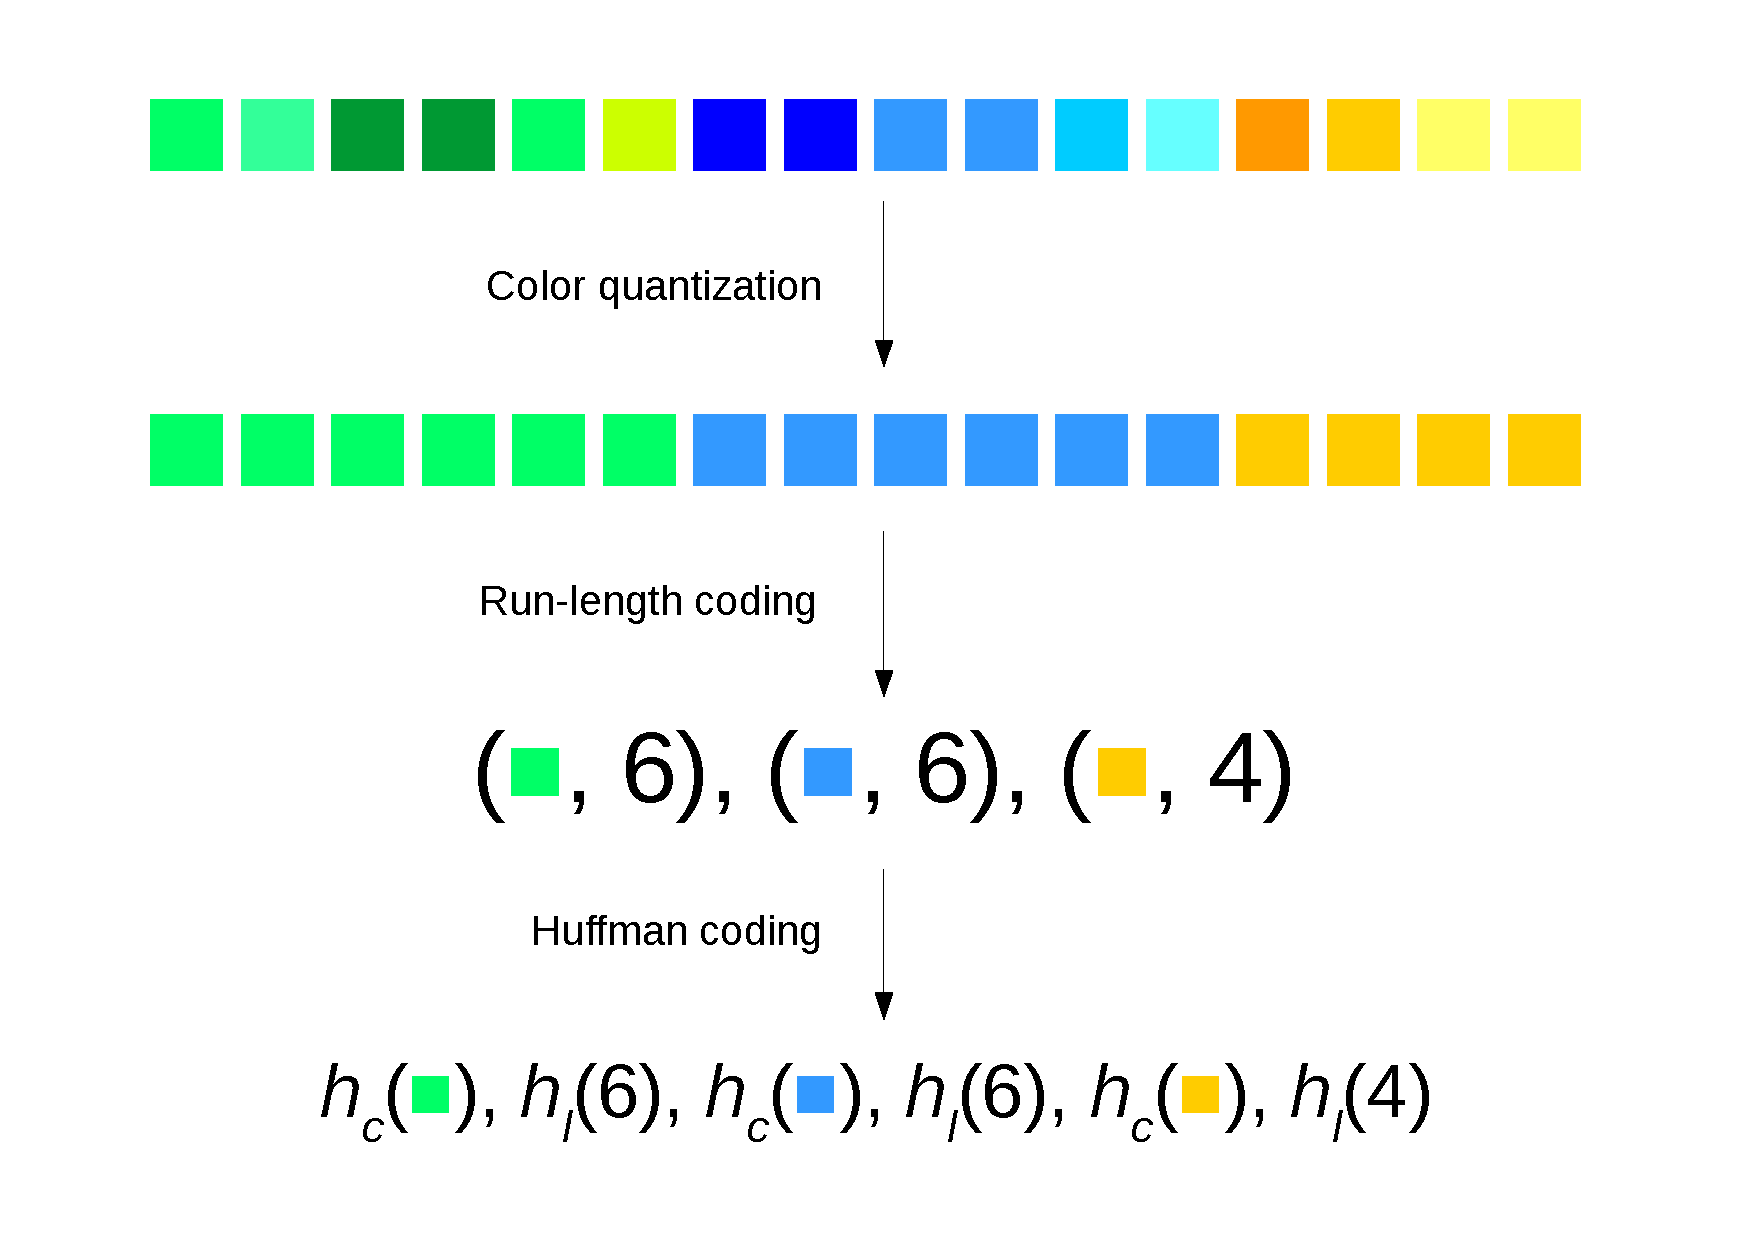
\includegraphics[width=1.0\textwidth]{img1/compression_scheme}
    \end{center}
\end{frame}

\begin{frame}{Huffman coding preprocessing}
    \begin{block}{On colors}
        \begin{itemize}
            \item Color quantization reduces the color space size from \SI{16}{M} to \SI{4}{K}.
            \begin{itemize}
                \item Keeps code length reasonable
                \item Reasonable hardware size (FPGA)
                \item Improves compression rate
                \item Efficient encoding
                \item Lightning scheme designed to behave well with color quantization
            \end{itemize}
        \end{itemize}
    \end{block}

    \begin{block}{On lengths}
        \begin{itemize}
            \item Smart lengths choice (1, 2, ..., 16, 32, 64, ..., 4096)
            \begin{itemize}
                \item Keeps code length reasonable (max. 6 bits)
                \item Reasonable hardware size (FPGA)
            \end{itemize}
        \end{itemize}
    \end{block}
\end{frame}

\begin{frame}{Performances}
    \begin{block}{Compression rate}
        \begin{itemize}
            \item Uncompressed : \SI{600}{kB/frame}
            \item Compressed without picture : \SI{4}{kB/frame}
            \item Compressed with picture : \SI{15}{kB/frame} 
        \end{itemize}
    \end{block}
        
    \begin{block}{Speed}
        \begin{itemize}
            \item Coding : \SI{3}{ms} per frame
            \item Decoding : 1 pixel per clock cycle (at \SI{33}{\mega\hertz})
        \end{itemize}
    \end{block}
\end{frame}

\section{SPI communication}
\begin{frame}{Plan of the presentation}
    \begin{center}
        \includegraphics[width=0.8\textwidth]{img1/block_global_device_highlight_spi_cropped}
    \end{center}
\end{frame}

\begin{frame}{SPI state machine}
    \begin{center}
        \includegraphics[width=0.5\textwidth]{img1/spi_state_machine_cropped}
    \end{center}

    \begin{itemize}
        \item \SI{5}{Mb/s}
        \item Burst mode, very low protocol overhead, chip select not released
        \item Connected to multiple RAMs through an MMU
    \end{itemize}
\end{frame}

\section{Display manager}
\begin{frame}{Plan of the presentation}
    \begin{center}
        \includegraphics[width=0.8\textwidth]{img1/block_global_device_highlight_display_cropped}
    \end{center}
\end{frame}

\begin{frame}{Hardware-controlled double-buffering}
    \begin{center}
        \includegraphics[width=1.0\textwidth]{img1/display_manager_cropped}
    \end{center}
    

\end{frame}

\section{Nios µC/OSII}
\begin{frame}{Plan of the presentation}
    \begin{center}
        \includegraphics[width=0.8\textwidth]{img1/block_global_device_highlight_nios_cropped}
    \end{center}
\end{frame}

\begin{frame}{µC/OSII functionnalities}
    \begin{center}
        \includegraphics[width=0.8\textwidth]{img1/tasks_mC_cropped}
    \end{center}
\end{frame}

\section{Player pictures acquisition}

\begin{frame}{Pipeline}
    \begin{center}
        \includegraphics[width=0.8\textwidth]{img1/block_pictures_cropped}
    \end{center}
\end{frame}

\begin{frame}[standout]
    Conclusion
\end{frame}

\begin{frame}[standout]
    Questions?
\end{frame}

\appendix

%\begin{frame}[allowframebreaks]{References}
%	\nocite{*}
%  	\bibliography{biblio}
%  	\bibliographystyle{abbrv}
%\end{frame}

\end{document}
